\documentclass[tikz,border=5pt]{standalone}
\usepackage{amsmath}
\usetikzlibrary{arrows.meta,positioning,calc,fit}
\definecolor{psablue}{RGB}{74,126,176}
\definecolor{addred}{RGB}{225,82,79}
\definecolor{normgreen}{RGB}{104,171,165}
\definecolor{gainyellow}{RGB}{235,190,73}
\definecolor{shufflepurple}{RGB}{164,115,156}
\definecolor{taubrown}{RGB}{151,107,69}
\tikzset{
  block/.style={draw=black!65, rounded corners=2pt, minimum width=20mm,
    minimum height=8mm, align=center, fill=white, font=\sffamily\small},
  state/.style={draw=black!65, circle, minimum size=7mm, fill=white,
    font=\sffamily\scriptsize},
  arrow/.style={-{Latex[length=2.2mm]}, semithick, draw=black!70},
  memory/.style={-{Latex[length=2.2mm]}, semithick, dashed},
  label/.style={font=\sffamily\small, align=left},
  note/.style={font=\sffamily\small, align=center, text width=47mm},
  tag/.style={font=\sffamily\bfseries\small, anchor=west}
}
\begin{document}
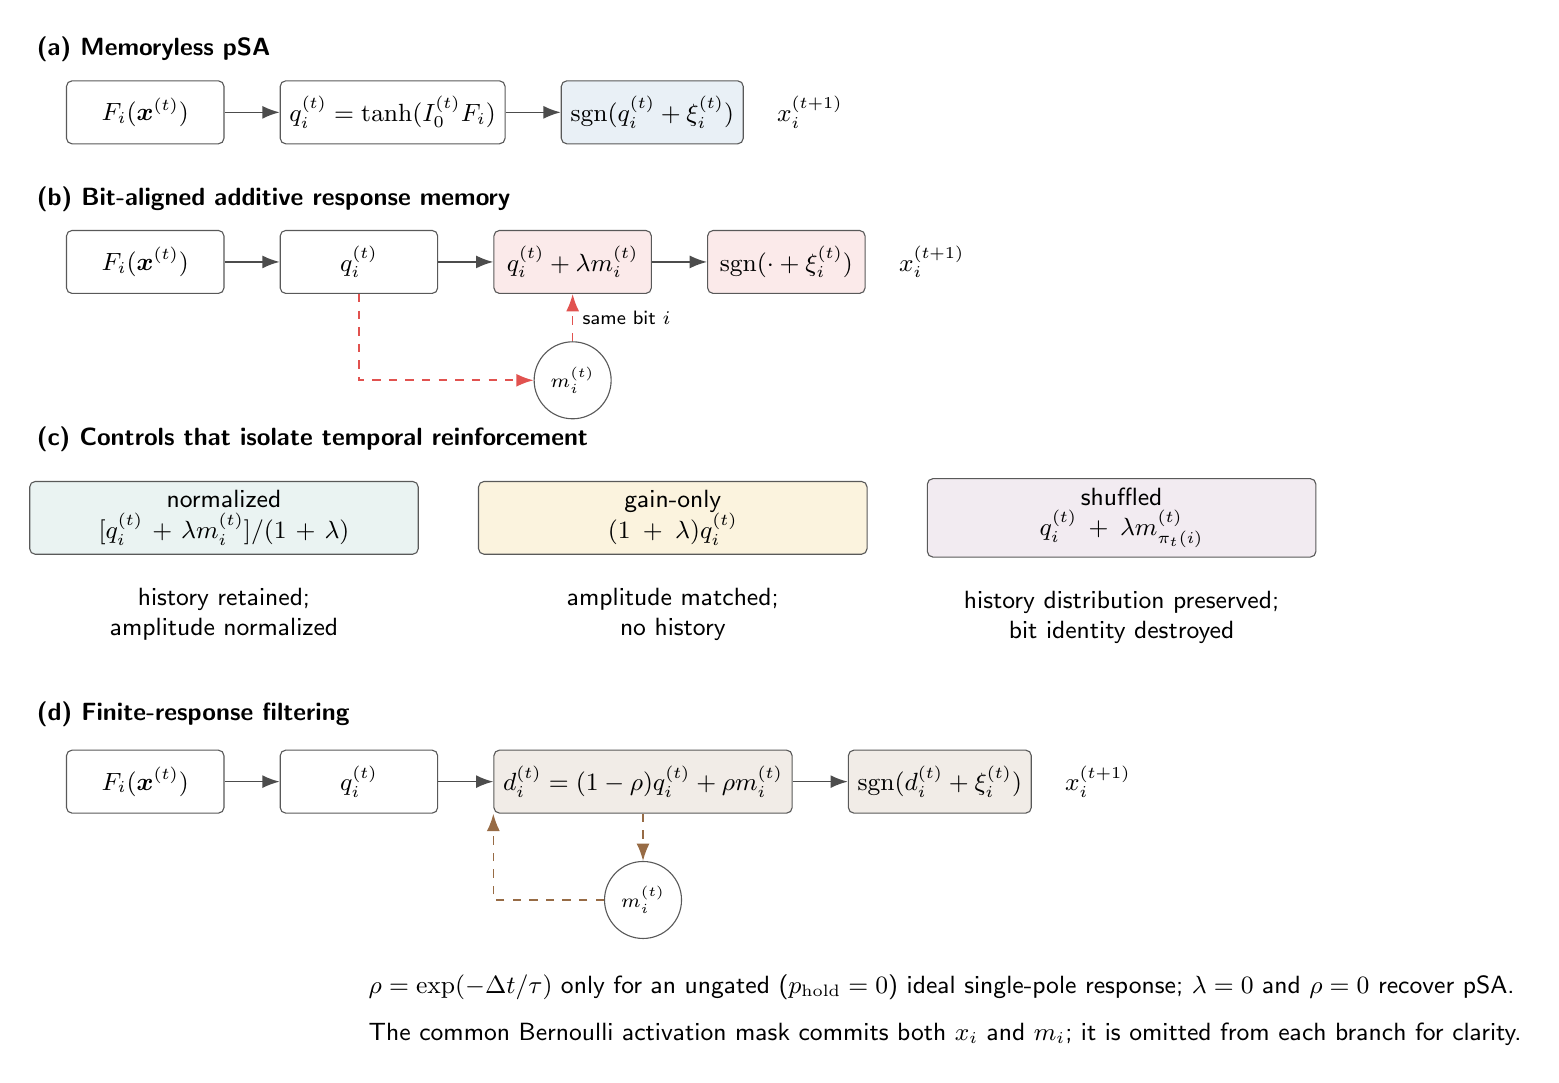
\begin{tikzpicture}[x=1cm,y=1cm]
  \node[tag] at (0,3.9) {(a) Memoryless pSA};
  \node[block] (field0) at (1.5,3.1) {$F_i(\boldsymbol{x}^{(t)})$};
  \node[block, right=7mm of field0] (tanh0) {$q_i^{(t)}=\tanh(I_0^{(t)}F_i)$};
  \node[block, right=7mm of tanh0, fill=psablue!12] (sample0) {$\operatorname{sgn}(q_i^{(t)}+\xi_i^{(t)})$};
  \draw[arrow] (field0)--(tanh0); \draw[arrow] (tanh0)--(sample0);
  \node[label, right=3mm of sample0] {$x_i^{(t+1)}$};

  \node[tag] at (0,2.0) {(b) Bit-aligned additive response memory};
  \node[block] (field1) at (1.5,1.2) {$F_i(\boldsymbol{x}^{(t)})$};
  \node[block, right=7mm of field1] (tanh1) {$q_i^{(t)}$};
  \node[block, right=7mm of tanh1, fill=addred!12] (sum1) {$q_i^{(t)}+\lambda m_i^{(t)}$};
  \node[block, right=7mm of sum1, fill=addred!12] (sample1) {$\operatorname{sgn}(\cdot+\xi_i^{(t)})$};
  \node[state, below=6mm of sum1] (mem1) {$m_i^{(t)}$};
  \draw[arrow] (field1)--(tanh1); \draw[arrow] (tanh1)--(sum1); \draw[arrow] (sum1)--(sample1);
  \draw[memory, draw=addred] (tanh1.south) |- (mem1.west);
  \draw[memory, draw=addred] (mem1.north) -- node[right,font=\sffamily\scriptsize] {same bit $i$} (sum1.south);
  \node[label, right=3mm of sample1] {$x_i^{(t+1)}$};

  \node[tag] at (0,-1.05) {(c) Controls that isolate temporal reinforcement};
  \node[block, fill=normgreen!14, text width=47mm] (norm) at (2.5,-2.05) {normalized\\$[q_i^{(t)}+\lambda m_i^{(t)}]/(1+\lambda)$};
  \node[block, fill=gainyellow!18, text width=47mm] (gain) at (8.2,-2.05) {gain-only\\$(1+\lambda)q_i^{(t)}$};
  \node[block, fill=shufflepurple!14, text width=47mm] (shuffle) at (13.9,-2.05) {shuffled\\$q_i^{(t)}+\lambda m_{\pi_t(i)}^{(t)}$};
  \node[note, below=3mm of norm] {history retained;\\amplitude normalized};
  \node[note, below=3mm of gain] {amplitude matched;\\no history};
  \node[note, below=3mm of shuffle] {history distribution preserved;\\bit identity destroyed};

  \node[tag] at (0,-4.55) {(d) Finite-response filtering};
  \node[block] (field2) at (1.5,-5.4) {$F_i(\boldsymbol{x}^{(t)})$};
  \node[block, right=7mm of field2] (tanh2) {$q_i^{(t)}$};
  \node[block, right=7mm of tanh2, fill=taubrown!13] (filter) {$d_i^{(t)}=(1-\rho)q_i^{(t)}+\rho m_i^{(t)}$};
  \node[block, right=7mm of filter, fill=taubrown!13] (sample2) {$\operatorname{sgn}(d_i^{(t)}+\xi_i^{(t)})$};
  \node[state, below=6mm of filter] (mem2) {$m_i^{(t)}$};
  \draw[arrow] (field2)--(tanh2); \draw[arrow] (tanh2)--(filter); \draw[arrow] (filter)--(sample2);
  \draw[memory, draw=taubrown] (filter.south) -- (mem2.north);
  \draw[memory, draw=taubrown] (mem2.west) -| (filter.south west);
  \node[label, right=3mm of sample2] {$x_i^{(t+1)}$};
  \node[label, below=22mm of tanh2, anchor=west] {$\rho=\exp(-\Delta t/\tau)$ only for an ungated ($p_{\mathrm{hold}}=0$) ideal single-pole response; $\lambda=0$ and $\rho=0$ recover pSA.};
  \node[label, below=28mm of tanh2, anchor=west] {The common Bernoulli activation mask commits both $x_i$ and $m_i$; it is omitted from each branch for clarity.};
\end{tikzpicture}
\end{document}
